\documentclass{sigchi}

% Use this command to override the default ACM copyright statement (e.g. for preprints). 
% Consult the conference website for the camera-ready copyright statement.


%% EXAMPLE BEGIN -- HOW TO OVERRIDE THE DEFAULT COPYRIGHT STRIP -- (July 22, 2013 - Paul Baumann)
% \toappear{Permission to make digital or hard copies of all or part of this work for personal or classroom use is 	granted without fee provided that copies are not made or distributed for profit or commercial advantage and that copies bear this notice and the full citation on the first page. Copyrights for components of this work owned by others than ACM must be honored. Abstracting with credit is permitted. To copy otherwise, or republish, to post on servers or to redistribute to lists, requires prior specific permission and/or a fee. Request permissions from permissions@acm.org. \\
% {\emph{CHI'14}}, April 26--May 1, 2014, Toronto, Canada. \\
% Copyright \copyright~2014 ACM ISBN/14/04...\$15.00. \\
% DOI string from ACM form confirmation}
%% EXAMPLE END -- HOW TO OVERRIDE THE DEFAULT COPYRIGHT STRIP -- (July 22, 2013 - Paul Baumann)


% Arabic page numbers for submission. 
% Remove this line to eliminate page numbers for the camera ready copy
\pagenumbering{arabic}


% Load basic packages
\usepackage{balance} % to better equalize the last page
\usepackage{graphics} % for EPS, load graphicx instead
\usepackage{times}  % comment if you want LaTeX's default font
\usepackage{url}   % llt: nicely formatted URLs
\usepackage{listings}
\usepackage{color}

\definecolor{mygreen}{rgb}{0,0.6,0}
\definecolor{mygray}{rgb}{0.5,0.5,0.5}
\definecolor{mymauve}{rgb}{0.58,0,0.82}
\definecolor{black}{rgb}{0,0,0}

\lstset{ %
  backgroundcolor=\color{white},   % choose the background color; you must add \usepackage{color} or \usepackage{xcolor}
  basicstyle=\scriptsize\ttfamily,        % the size of the fonts that are used for the code
  breakatwhitespace=false,         % sets if automatic breaks should only happen at whitespace
  breaklines=true,                 % sets automatic line breaking
  captionpos=b,                    % sets the caption-position to bottom
  commentstyle=\color{mygreen},    % comment style
  deletekeywords={...},            % if you want to delete keywords from the given language
  escapeinside={\%*}{*)},          % if you want to add LaTeX within your code
  extendedchars=true,              % lets you use non-ASCII characters; for 8-bits encodings only, does not work with UTF-8
  frame=single,                    % adds a frame around the code
  keepspaces=true,                 % keeps spaces in text, useful for keeping indentation of code (possibly needs columns=flexible)
  keywordstyle=\color{blue},       % keyword style
  %language=Octave,                 % the language of the code
  morekeywords={*,...},            % if you want to add more keywords to the set
  numbers=left,                    % where to put the line-numbers; possible values are (none, left, right)
  numbersep=5pt,                   % how far the line-numbers are from the code
  numberstyle=\tiny\color{mygray}, % the style that is used for the line-numbers
  rulecolor=\color{black},         % if not set, the frame-color may be changed on line-breaks within not-black text (e.g. comments (green here))
  showspaces=false,                % show spaces everywhere adding particular underscores; it overrides 'showstringspaces'
  showstringspaces=false,          % underline spaces within strings only
  showtabs=false,                  % show tabs within strings adding particular underscores
  stepnumber=2,                    % the step between two line-numbers. If it's 1, each line will be numbered
  stringstyle=\color{black},     % string literal style
  tabsize=2,                       % sets default tabsize to 2 spaces
  title=\lstname                   % show the filename of files included with \lstinputlisting; also try caption instead of title
}

% llt: Define a global style for URLs, rather that the default one
\makeatletter
\def\url@leostyle{%
 \@ifundefined{selectfont}{\def\UrlFont{\sf}}{\def\UrlFont{\small\bf\ttfamily}}}
\makeatother
\urlstyle{leo}


% To make various LaTeX processors do the right thing with page size.
\def\pprw{8.5in}
\def\pprh{11in}
\special{papersize=\pprw,\pprh}
\setlength{\paperwidth}{\pprw}
\setlength{\paperheight}{\pprh}
\setlength{\pdfpagewidth}{\pprw}
\setlength{\pdfpageheight}{\pprh}

% Make sure hyperref comes last of your loaded packages, 
% to give it a fighting chance of not being over-written, 
% since its job is to redefine many LaTeX commands.
\usepackage[pdftex]{hyperref}
\hypersetup{
pdftitle={SIGCHI Conference Proceedings Format},
pdfauthor={LaTeX},
pdfkeywords={SIGCHI, proceedings, archival format},
bookmarksnumbered,
pdfstartview={FitH},
colorlinks,
citecolor=black,
filecolor=black,
linkcolor=black,
urlcolor=black,
breaklinks=true,
}

% create a shortcut to typeset table headings
\newcommand\tabhead[1]{\small\textbf{#1}}


% End of preamble. Here it comes the document.
\begin{document}

\title{DressCode: Tools and Activities to Engage Youth in Algorithmic Craft}

\numberofauthors{3}
\author{
 \alignauthor 1st Author Name\\
  \affaddr{Affiliation}\\
  \affaddr{Address}\\
  \email{e-mail address}\\
  \affaddr{Optional phone number}
 \alignauthor 2nd Author Name\\
  \affaddr{Affiliation}\\
  \affaddr{Address}\\
  \email{e-mail address}\\
  \affaddr{Optional phone number}  
 \alignauthor 3rd Author Name\\
  \affaddr{Affiliation}\\
  \affaddr{Address}\\
  \email{e-mail address}\\
  \affaddr{Optional phone number}
}

\maketitle

\begin{abstract}
%Programing is a singular creative tool with the potential to support personal expression. Unfortunately, many people who are new to programing view it as a highly specialized, difficult and inaccessible skill that is only relevant for career paths in science, engineering, or business fields. Despite this perception, programing enables novel forms of creative expression and communication in the medium of computation. Visual and physical art, craft, and design are interrelated domains that offer exciting possibilities when extended by computation. By forging strong connections between the skill of programming and the construction of personally relevant physical objects, it may be possible to foster meaningful creative experiences in computation and making for non-professionals. The combination of computational design, digital fabrication, and hand craft to create functional artifacts offers an opportunity to make programing compelling for people with an interest in craft-sensitive forms of making. I define the synthesis of these fields with the term \textit{algorithmic craft}. DressCode is a software tool that attempts to make the practice of algorithmic craft accessible for novice programers. This document describes the design of DressCode and the results of in engaging people in the creation of objects that are imagined by the mind, designed with programming, formed by machines, and primitived by hand.
\end{abstract}

\keywords{
	Guides; instructions; author's kit; conference publications;
	keywords should be separated by a semi-colon.
	\textcolor{red}{Mandatory section to be included in your final version.}
}

\category{H.5.m.}{Information Interfaces and Presentation (e.g. HCI)}{Miscellaneous}

See: \url{http://www.acm.org/about/class/1998/}
for more information and the full list of ACM classifiers
and descriptors. 
\textcolor{red}{Mandatory section to be included in your
final version. On the submission page only the classifiers'
letter-number combination will need to be entered.}

\section{Introduction}
Computation is a driving force in our world. The recognition of the importance of computation to both national and international industry and advancement has resulted in the STEM Education Initiative, a national drive to engage young people in topics of math, science, engineering, and computer science \cite{stemReport}. Proposed K-12 computer science educational curriculums are aimed at teaching students the core components of computation and programing, as well as fostering sustained interest in a broad range of computer science professions \cite{k12ModelCur}. These approaches explore digital applications of computer science that will appeal to young people, including game development, digital media manipulation, and web development. Parallel to the growth of youth STEM initiatives is the recognition of the educational potential of the Maker movement, which has produced a growing number of youth-oriented maker initiatives. These programs seek to create opportunities for young people to participate in hands-on learning through making \cite{makerinitiatives}, and conduct research on how hands-on-learning can be integrated with educational policy and practice \cite{maketolearn}. Many youth maker initiatives are designed to connect directly to STEM educational objectives, by connecting making with principles in science, technology and math; however these initiatives also have great potential to connect with the arts. As researchers, we believe computation can serve as a powerful tool for creative disciplines. When applied to the arts, programming offers different paradigms for creation and new methods of problem solving. We see an opportunity to support young people in art-oriented programing by connecting computation to making. Specifically, we seek to support youth in the combined use of computational design and traditional arts and crafts for the production of functional and decorative physical artifacts. We use term \textit{algorithmic craft} as a way of describing this collective practices. % something about how learning progrmaing is not the key goal. 
%examples of craft.

Combining computational design and handcraft raises many interesting questions:
What are the important design principles to consider when creating programming environments for physical design? How do we compellingly link textual code with visual designs, and what are the appropriate intersection points between textual manipulation and visual manipulation? What support is required to help people move back and forth from programming to building real objects in a way that is comfortable, expressive, and pleasurable? How can we remove the technical challenges involved in translating code into an object that can be successfully fabricated, but still support a wide variety of design styles, aesthetics, and approaches? Finally, how can we interlink the often disparate processes of physical prototyping with digital design and programming in a way that creatively reinforces both physical and virtual modes of working?

To explore these questions we developed a software tool called DressCode, to enable young novice programers to participate in computational design. We designed and implementation of a set of algorithmic craft activities in which high-school students used DressCode in conjunction with traditional forms of hand-craft to produce personal artifacts. Throughout our description and analysis of these experiences, we discuss design factors that enable young people to use computation in ways that emphasize pleasure, intellectual engagement, and utility in the service of personal expression.

\section{Algorithmic Craft}
In order to illustrate the creative potential of algorithmic craft, it is useful to examine the key affordances of computational design and craft and how they can be combined into a single practice. In computational design, the abstract qualities of computer programming provide a powerful way of thinking about design. Similarly, computational design can be applied to any design domain, be it physical, visual, sonic, or interactive. Our focus focus in computational design is the process of using computational processes to create visual forms and patterns. Although individual applications of computational design often consider material properties that are relevant to a specific domain, computational design does not possess an inherent connection to the material world. Craft on the other hand is closely linked to materiality. Craftspeople work in close contact with the physical world and craft artifacts and processes are directly informed by material properties. 
\subsection{Affordances of Computational Design}
\begin{itemize}
\item \textbf{Precision:} Computation supports high levels of numerical precision.
\item \textbf{Visual Complexity:} Computational design allows for the creation and transformation of complex patterns and structures through rapid automation and iteration which allows for the combination and manipulation of large numbers of simple elements in a structured manner. 
\item \textbf{Generativity and Self-Similar Forms} Computation allows for the programmer to create algorithms that allow for the computer to autonomously produce unique and unexpected designs.
\item \textbf{Parameterization:} Computation allows users to specify a set of degrees of freedom and constraints of a model and then adjust the values of the degrees of freedom while maintaining the constraints of the original model.
\item \textbf{Documentation and remixing:} Computationally generated designs are generated by a program which can be modified by other designers, and serve as a form of documentation of the design process. 
\end{itemize}	
Computational design also contains a number of unique challenges:
\begin{itemize}
\item \textbf{Formalizing complex problems} As design problems grow in complexity, formalizing the problem in a manner that can be expressed programmatically becomes challenging. 
\item \textbf{Creating singularities:} A designer will often choose to deviate from a set pattern or structure at specific points in order to create a special emphasis in the area of deviation. Because computational design is governed by a systematized ruleset, the methods of breaking these rules at arbitrary points are often unclear or tedious to implement. 
\item \textbf{Selecting a final design:} Computational design gives the designer the ability to produce extremely large numbers of solutions to a single design problem. While this is useful in situations where multiple solutions are required, when a single design must be chosen, the process of deciding on a solution is difficult, especially if the decision is based on aesthetic criteria.
\end{itemize}

\subsection{Affordances of Craft}
The cultural connotations of craft have varied throughout history, however forms of craft have endured, both as a recreational pursuit, and as set of valued artisanal practices. Below we describe the specific aspects that are integral to algorithmic craft.
\begin{itemize}
\item \textbf{Materiality:} Craft involves the manipulation of physical materials by hand, which is often an intuitive physical process. The decisions made in the craft process are altered by the feel of working with the material. 

\item \textbf{Pleasure:} Fundamental to traditional conceptions of arts and crafts is the idea of pleasure in working with one's hands \cite{abstracting_craft}. This emphasis on pleasure is retained in conceptions of professional and amateur craft practices today.

\item \textbf{Unification of form and function:} Although not all craft is functional, many forms of traditional craft can applied the creation of useful objects. In addition craft often emphasizes the importance of beauty in the form and ornamentation of objects. Well crafted artifacts frequently demonstrate the successful unification of aesthetics and utility.

\item \textbf{Craftsmanship:} Put in a description of craftsmanship
\end{itemize}

\subsection{The potential of Algorithmic Craft}
The combination of computational design and craft offers the opportunity to produce pieces that are connected to a distinct space, time and process, and that are primitived by material properties, while incorporating patterns and forms made possible through computational processes.Objects that emerge from a combined practice of digital fabrication and craft are often characterized by their physical craftsmanship, technical mastery, and exceptional aesthetic. Practitioners in this space blur the boundaries between engineer, designer, and artisan. One of the advantages of merging craft and digital fabrication is that it ensures that machine-produced artifacts retain their personal history. Combining computational design and craft also offers the opportunity to engage people with interest in craft in the use of computational tools.

\subsection{Digital to Physical Translation}
In order to connect the digital artifacts of computational design with the physical world of craft, some form of transition is needed between the digital and the physical. Digital fabrication technology provides one method of connecting the abstraction of computational design and the material domain of craft by converting digital designs to physical forms. Digital fabrication technology ranges from the additive processes of 3D printing, to the subtractive manufacturing techniques of laser cutting, CNC mlling and vinyl cutters. Subtractive fabrication technology often corresponds well with craft processes Unlike most 3D printing technology, subtractive processes can work with a wide range of materials \cite{dunn}.

Time is an important quality of crafting. Handcrafted artifacts often require a great deal of time to complete and involve repetitive tasks. Because the process of crafting is often pleasurable and contemplative, many people look forward to spending time productively engaged with their hands. In algorithmic craft, the role of digital fabrication is not to speed up craft, but to facilitate the translation of computational forms to physical materials. These physical forms, in turn, can be primitived through craft processes, and imbue computational designs with individuality, utility, and temporality. Several forms of digital fabrication machines are capable of producing forms that are suitable for both expert and novice levels of handcraft. Because subtractive fabrication technologies work with materials like wood, paper, and fabric, they support the creation of objects that are readily primitived by the human hand. Laser-cut parts can be sanded, polished, painted, sewn, or folded after they emerge from the machine. Vinyl cutters also can be used on cloth and paper. They also produce patterns in adhesive vinyl that can be applied to screens for for screen printing. Laser cutters and vinyl cutters also fabricate at a faster rate than 3D printers or milling machines, and permit a higher tolerance for error during the craft process because it is feasible to re-cut damaged parts. Inkjet printers can also function as a form of digital fabrication, as they can print on cloth, or transparencies used in screen printing...

\subsection{Challenges in access and application}
primary barriers being:
perceptual: people don't know you can use programing for physical making and craft
intellectual: learning the unique affordances of computation and applying them in personally meaningful ways
technical- challenge of using programing for design
Focused on software design for the technical, activity design for the perceptual

\section{Related Software Tools}
\subsection{Professional Tools}
\subsection{Entry-level Programming Environments}
\subsection{Entry-level CAD Tools}

\section{DressCode Software Design}
DressCode is a 2D computational design tool aimed at novice programers. The primary objectives in the design of DressCode were to reduce the technical challenges of computational design, to foster independent and deliberate design decisions, and to assist in the creation of designs that were viable for craft applications. Although the name of the tool reflects an emphasis on wearables and fashion, as an application DressCode is general purpose, and can be applied to many forms of algorithmic craft. The software is comprised of the following elements: A custom programing language and drawing application programing interface (API), an integrated development environment, and a graphic user interface design tool. 
\begin{center}
\begin{figure}[h!]
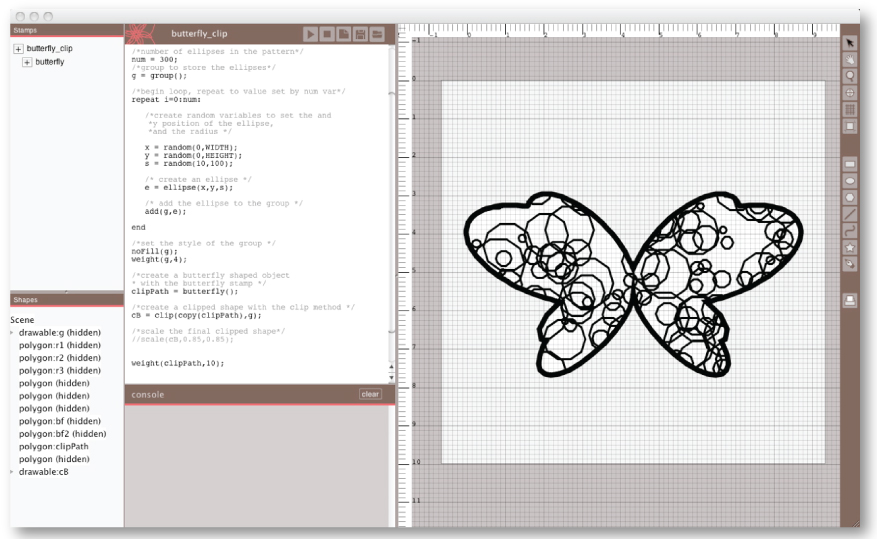
\includegraphics[width=\columnwidth]{images/dresscode_interface.jpg}
\caption{The DressCode software}
\label{fig:dresscode_interface}
\end{figure}
\end{center}
\subsection{Interface}
The interface of DressCode is divided into two sections: a design panel on the left and a coding panel on the right. The design panel approximates many of the features of a digital graphic design tool, with rulers, a grid, a drawing board, and a graphic tool menu. The drawing board defines the coordinate system referenced by the drawing API with the upper left hand corner corresponding to (0,0) in cartesian coordinates. Users can resize the drawing board and set the units to inches or millimeters at any point during the design process by selecting the drawing board icon in the tool menu. Similarly, the pan and zoom tools allow the user to navigate around the drawing board. The print tool opens a dialog that allows the user to export their current design in a vector format for output through digital fabrication. 

The coding panel contains a primary window for entering text, and an output console for print output and error reporting. It also contains two additional panels, a declarative listing view, and the Stamp menu. Both of these panels are discussed in detail in the Graphic Tools section. A toolbar on top of the coding panel allows the user to save their existing program, open a program, or run their current program. When a program is run, the resulting design is displayed in the design panel. The DressCode programming language is interpreted with semantic functionality that is simulated through a Java-based library. For most programs, the interpretation process is instantaneous; however, some programs with complex operations require several seconds to be executed. Early in the development process, we experimented with automatic interpretation, wherein the design would be automatically updated as changes were made to the code. Early user testing demonstrated that this process produced a great deal of frustration, and people explicitly requested control over running their program and updating their design.

%\begin{center}
%\begin{figure*}[h!]
%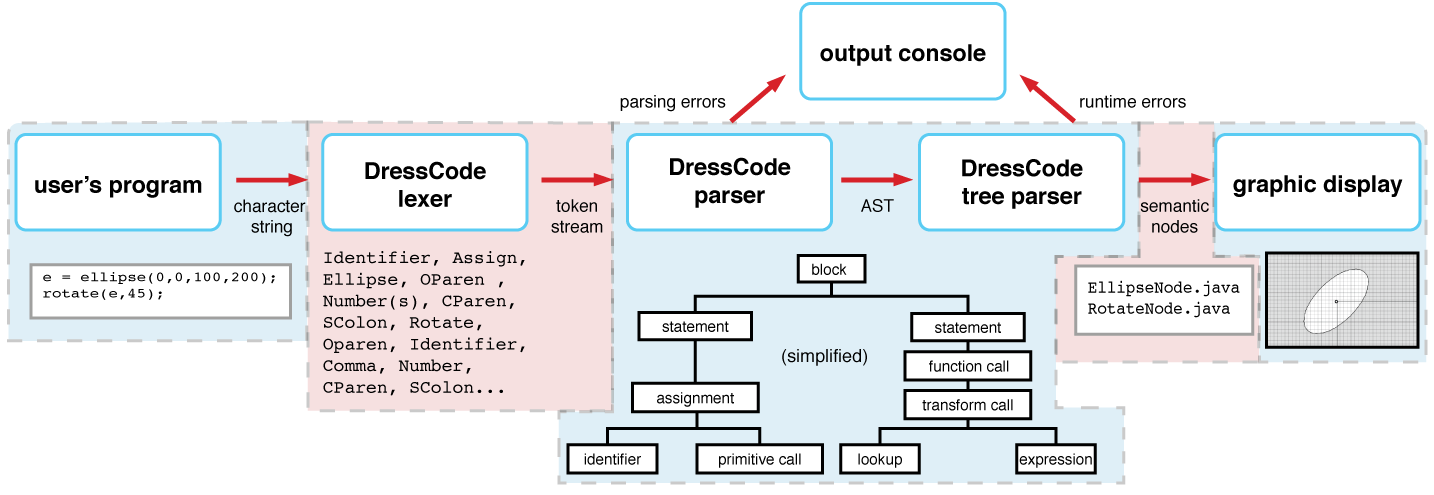
\includegraphics[width=\textwidth]{images/interpreter_structure_horz.png}
%\caption{Interpreter structure}
%\label{fig:interpreter_structure}
%\end{figure*}
%\end{center}

\subsection{Programming Language and Drawing API}
DressCode features a custom textual programing language with native 2D drawing functionality\footnote{A full specification of the DressCode language and API is available at: \url{http://jacobsj.scripts.mit.edu/dresscode/index.php?title=Drawing_API_Reference}}. The language supports conventional datatypes including numbers, strings, booleans, and lists, and also supports drawing primitive datatypes such as ellipses, rectangles and polygons, as well as groups of primitives. The language also contains support for basic expressions, as well as conditionals, loops and user-defined functions. DressCode is dynamically typed in order to reduce syntactic challenges for people new to textual programing. DressCode determines how to treat the data assigned to an identifier based on context and identifiers can be assigned to datatypes that differ from their original assignment at any point. 

The DressCode drawing API is s formulated on an Object Oriented Programming (OOP) paradigm which enables users to create and manipulate collections of geometric primitives including points, lines, curves, polygons, ellipses, rectangles and imported SVG primitives. Shape primitives are initialized by calling the appropriate primitive method, and passing it a set of parameters designating the initial appearance of the primitive. For all primitives besides lines and curves, the first two parameters designate the coordinates of origin point of the primitive, and each primitive is drawn in the design panel relative to this central origin point. There is no ``draw" method for DressCode. Instead all primitives are automatically drawn in the order of their initialization. This was designed to make it as easy and immediate as possible to have a design appear on the screen. Objects can be selectively hidden with the hide method. 
 
All primitives in DressCode can be modified through two kinds transformation methods, Geometric and Stylistic. Geometric transformations allow  for primitives to be rotated, scaled or moved or combined with other primitives. All geometric transformations are performed relative to the origin of the primitive, unless otherwise specified. Rotation statements for example have an optional third parameter which specifies a point to rotate the primitive around. Stylistic transformations affect the appearance of a primitive, and can modify properties like fill and stroke color, stroke weight, and presence or absence of fill and stroke. Transformations on a primitive are performed by assigning an identifier to the primitive, and then calling the transformation method with the identifier. By using the transformation methods to manipulate primitives in a structured manner, it is possible to generate complex and interesting designs from simple forms. Through these methods, DressCode was intended to support the affordances of computational design, specifically precision, visual complexity, generativity and stylistic abstraction, in a way that was feasible for new practitioners.

 \begin{center}
\begin{figure}
\begin{lstlisting}
//repeat statement
repeat i=0:10:
ellipse(0,i*10,10,10); //draws a vertical row of 10 ellipses
end
\end{lstlisting}
%\caption{loop definitions}
%\label{fig:loops}
\end{figure}
\end{center}

As mentioned, DressCode also contains a set of transformation methods that allow primitive primitives to be combined with one-another via polygon boolean operations. Polygon booleans are widely used in CAD applications and are essential for many forms of digital fabrication because they allow for complex configurations of primitives to be combined into effective toolpaths. DressCode contains methods for performing unions, intersections, differences and either-or intersections between any two or more primitives. They can also expand strokes to filled polygon paths, enabling the translation of line art to a form that will maintain its appearance when fabricated. By positioning these operations as primary components of the DressCode, we attempted to create a programming language that produced forms that were applicable to fabrication as a direct result of the design process. 

As a method of organizing sets of primitives, DressCode contains a group datatype, which essentially is a specialized list for primitives. Groups can be initialized with a starting set of child primitives, or they can be initialized as empty, and then later have primitives added (or removed), from them. Groups automatically maintain an origin that is the average of all their children's origins. Geometric transformations performed on groups will relatively effect all of the primitives within the group; for example, if a group of polygons is moved to 0,0, then the origin of the group will become 0,0, with all polygons in the group being drawn relative to that new origin point. Groups can be multi-dimensional, and contain other groups. Stylistic transformations applied to groups will also be applied to each child. Groups also facilitate more advanced transformations. For example, it is possible to clip a group of primitives within the bounds of a single primitive to serve as a form of clipping mask, and a union can automatically be performed on all objects in a group with the merge method.

We chose to create a textual programing language for DressCode because we believe textual programing is well suited to transparent representations of computational design algorithms. In recognition of the challenges of first-time text programming, we also focused on creating intuitive forms of interaction and feedback to correspond with the DressCode language. These are inherent in the graphic drawing tools, which we discuss in the next section.
 
\subsection{Graphic Tools, Organizational Structures, and Visual Feedback Mechanisms}
\label{subsec:graphic_tools_test}
The drawing and manipulation tools in DressCode are designed to allow users to create and modify elements of their design through graphic selection. Collectively, the drawing functionality of the tools is similar to the functionality of many existing forms of  2D vector graphics software. The tools are distinguished from other graphics software tools because they maintain a direct symmetry with the DressCode programming language. Each tool correspond directly to a method in the drawing API. More importantly, the use of each tool automatically generates a corresponding textual statement in a user's program. This enables elements that are created graphically, to be immediately manipulated through textual programing, and is designed to encourage a natural flow between graphic drawing and textual programing throughout the design process. The toolset includes regular primitive creation tools (ellipse, rectangle, polygon, line curve), and an svg import tool. There is also a pen tool that allows for the creation of irregular forms. Use of the pen tool generates a list of points in the text program, and statement initializing a polygon with the list. Because of the symmetry between the DressCode graphic tools and the DressCode language, there is no functionality hidden from the user in the process of modifying elements graphically. The program that results from a graphically modified design is human readable, and can be frictionlessly shared with other users, or copied and pasted into other DressCode programs.

(figure:\ref{fig:auto_generated_code}). In addition to the primitive generation tools, there is also a selection tool, which allows for individual primitives and groups to be manually selected with the cursor, and moved to different points on the drawing board. When a primitive is moved for the first time, a textual move statement is inserted into the user's program, with the identifier for the moved primitive as the first argument. If the moved primitive does not have an identifier, the primitive declaration is wrapped by a move statement. For all subsequent moves of that primitive with the move tool, the inserted move statement is updated to reflect the new coordinates of the primitive. % insert image?

\begin{center}
\begin{figure}[h!]
%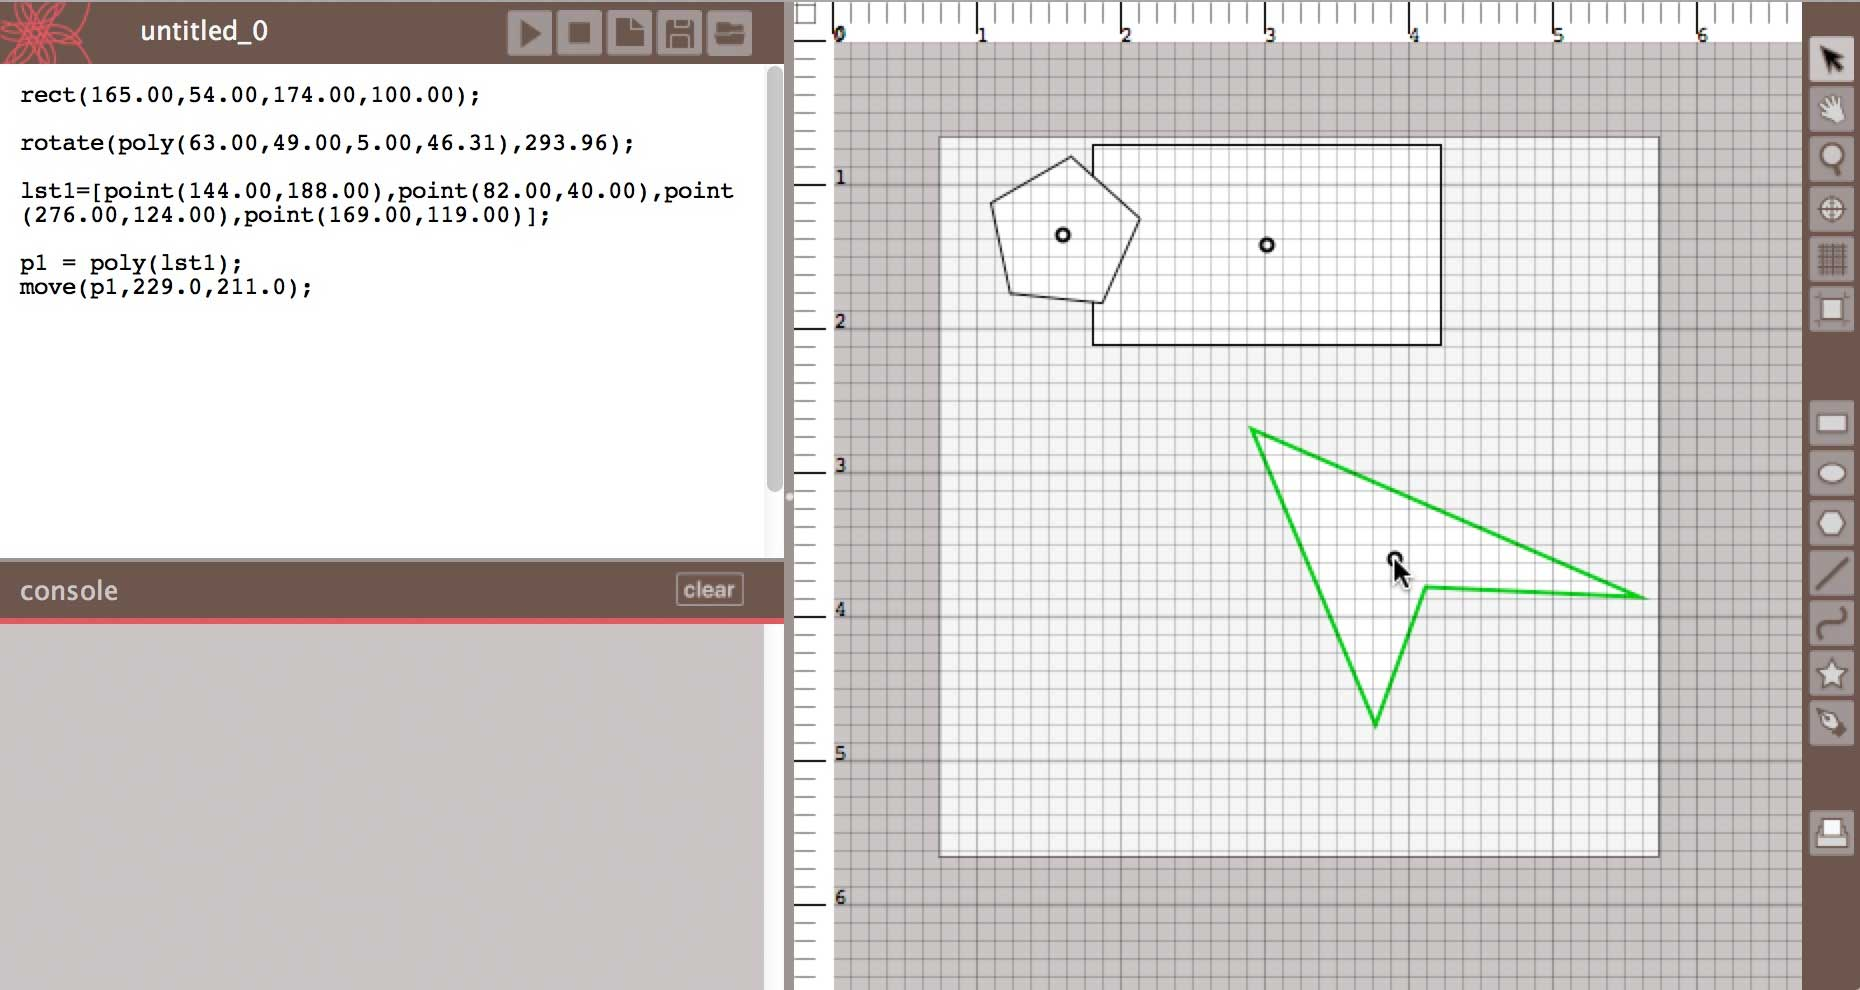
\includegraphics[width=\columnwidth]{images/auto_generated_code.jpg}
\caption{Graphically created polygon, rectangle, and irregular polygon, and corresponding automatically-generated code. The irregular polygon has just been moved with the selection tool.}
\label{fig:auto_generated_code}
\end{figure}
\end{center}

It is also possible to select primitives in the declarative view panel. The declarative view contains a listing of all primitives in the current design, listed by their type (polygon, line, ellipse etc.) and identifier. Child primitives of groups are shown as nested elements below the group. When a primitive is selected in the declarative view, the primitive is simultaneously selected (and highlighted) in the design view, and the line where the primitive was last modified in the textual program is highlighted (figure:\ref{fig:declarative_view}). This declarative view functionality is designed to provide visual feedback on how elements of a design connect to the a user's program, and provide a practical selection technique for selecting and modifying individual children within a complex group.


\begin{center}
\begin{figure}[h!]
%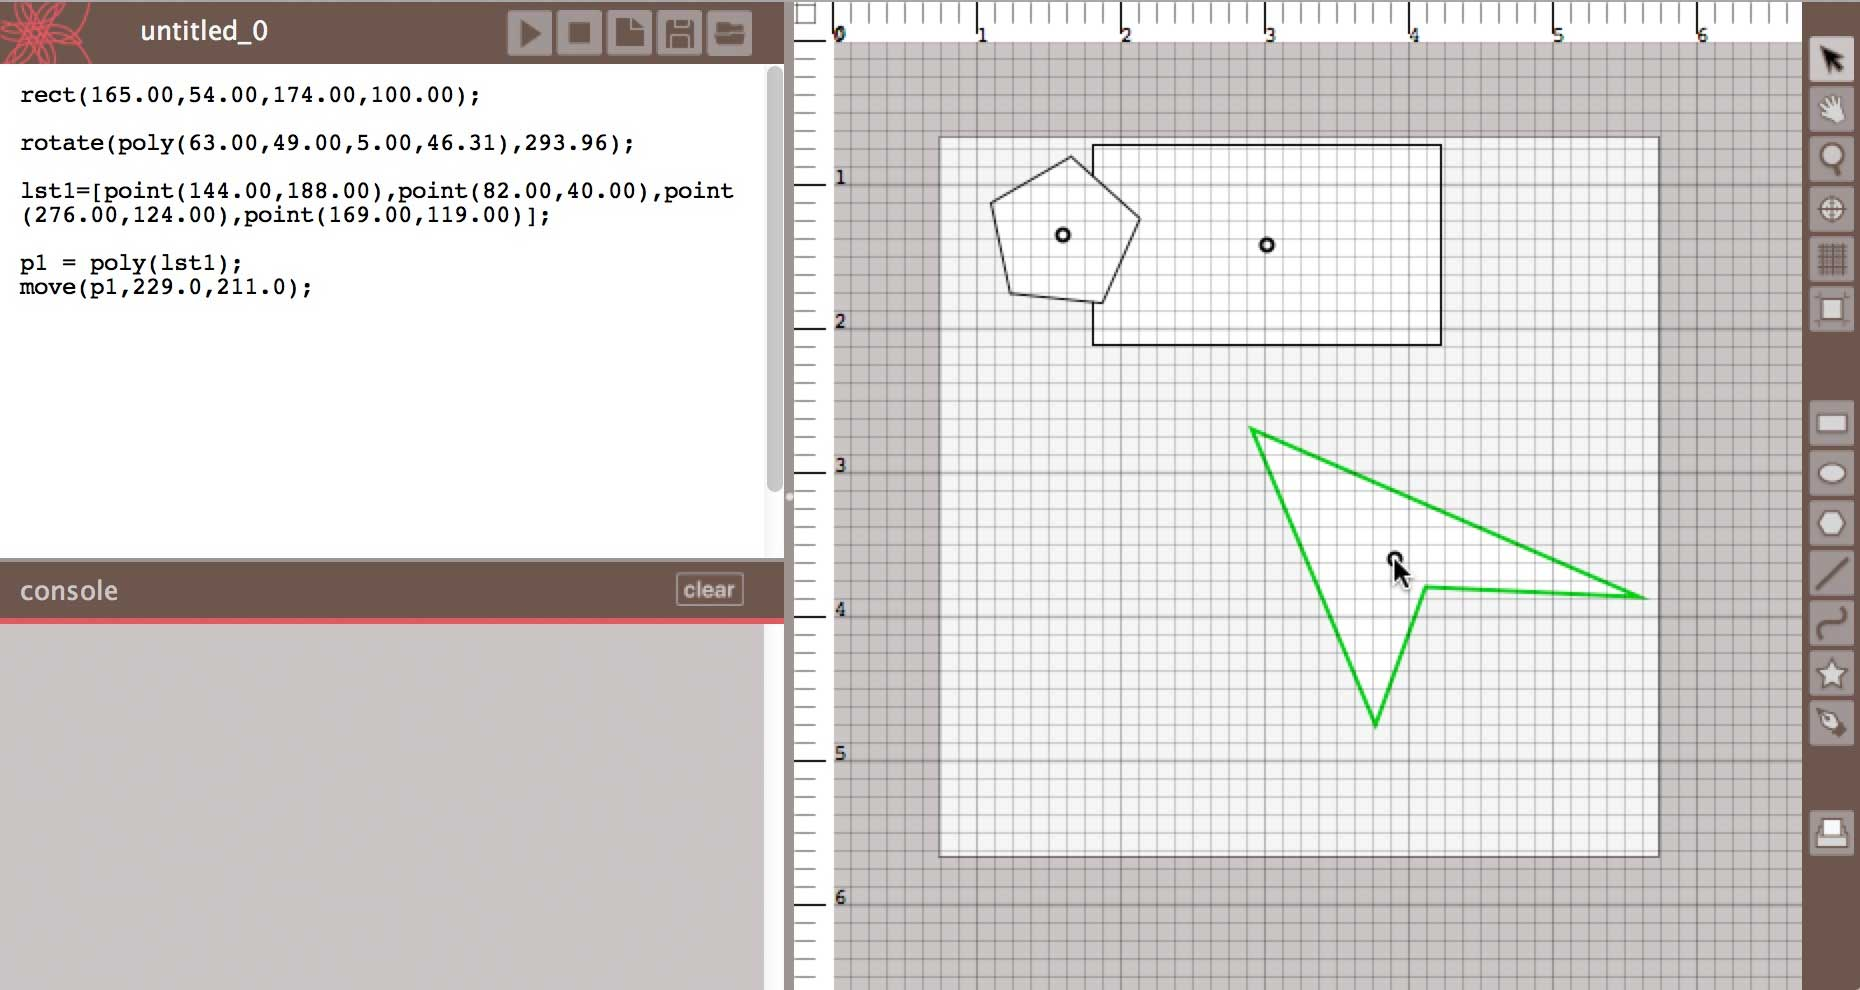
\includegraphics[width=\columnwidth]{images/auto_generated_code.jpg}
\caption{Declarative view with selected primitive}
\label{fig:declarative view}
\end{figure}
\end{center}

Finally, DressCode contains functionality to help people organize their code in the form of \textit{stamps}: auto-generated functions that return shape primitives. Two forms of stamps can be created: dynamic and static. Dynamic stamps are created by selecting a portion of code in a user's program. and then selecting the ``create stamp from selected code" option from the menu. A dynamic stamp will package the selected code in a function with a name specified by the user, and automatically return any primitives that are generated by the selected code in the last line of the function. Static stamps are created by graphically selecting a primitive or group of primitives with either the selection tool or the declarative view, and selecting the ``create static stamp from selected objects'' option. Similar to dynamic stamps, static stamps are a function with a user-defined name that return a copy of the primitive or group that is selected. Static stamps differ in that they contain an explicit representation of the selected primitives. Static stamps were created to assist in the process of generative design. For example, if you create a random collection of shapes using a random or noise method, the next time the program is run, a different random collection will be generated. If a user wishes to maintain a specific instance of a generative design, they can create a static stamp from it, which will contain methods describing that discreet representation of shapes. Stamps are listed the stamp menu and can be added to a user's primary program by selecting the ``+'' icon next to each stamp. The functionality of both static and dynamic stamps can be modified by the user, by selecting the stamp from the menu, which will display the stamp code in the primary code window in an editable format.


\section{Activity Design}
Domain-specific software is an important component of engaging youth in algorithmic craft; however it is equally important to appropriately design the context in which the software is applied. In this section, we discuss the primary components of our activity design, for which DressCode was the primary design tool. 
Because algorithmic craft combines aspects of computation, design and craft, we focused on an activity structure that would emphasize key components from each of these domains through three forms: learning, creation and reflection. 

\subsection{Learning}
Instruction in our algorithmic craft activities was divided between imparting conceptual understanding of the creative opportunities of algorithmic craft, and teaching practical skills necessary to act upon this knowledge. We presented participants with a conceptual overview of the core principles described in the Algorithmic Craft section, by sharing examples of professional projects that demonstrated these properties. We made a particular effort to link the properties of computational design to more familiar contexts, for example comparing parameterization to the process of creating a size-variable dress pattern for sewing, or using a coin flipping and drawing activity to demonstrate the properties of randomness and generativity.  To provide participants with the required technical knowledge for computational design, we conducted guided activities in programing in DressCode. For the programing lessons, we limited instruction to a specific design principle, such as radial symmetry or a random walk, and assisted participants through the process of creating their own algorithms that expressed this principle. For the craft skills, the instructors demonstrated the basic techniques of the craft activity, such as how to pull ink through a screen for screen printing, or how to set snaps into leather, and then gave participants the opportunity to try the process themselves.

\subsection{Creation}
Because one of the primary objectives for algorithmic craft activities is to have participants emerge with a completed artifact, we devoted the majority of activities to time for the participants to develop their designs and projects. Following each learning portion, we provided participants with time to experiment with the concepts or techniques that were covered, and develop their own interpretations. We also conducted longer-term design sessions that lasted 1-3 hours each and gave participants the opportunity for open-ended computational design. These sessions were supplemented by providing participants with DressCode examples which they could reference, modify or remix, quick syntax-reference sheets and an online code reference. Instructors were also present to help with programing questions, or offer design suggestions. The physical craft materials were made available to participants during the computational design sessions, so they could take their properties into account as they created their design. 

In the crafting and fabrication creation portions we emphasized hands-on practice and experimentation. Abundant test materials and extra supplies were provided to encourage participants to try crafting techniques until they were comfortable with the process. For activities that relied on digital fabrication, participants were given instruction on the use of the fabrication machines and then operated them independently under instructor supervision. We also encouraged participants to work collaboratively during the construction process, having groups of two or three people work to complete one individual's artifact, and then transition to working on the other's project. 

\subsection{Reflection}
At each stage of creation during an activity, we added an opportunity for reflection. Participants were introduced to the process of a design critique at the start of an activity, and then engaged in group critiques following each design and craft stage. For the critiques, we provided participants with  aesthetic and practical criteria to  guide their feedback. This ranged from composition and visual flow of a design, the level of complexity, the wearability of a design (how it would look when worn), and how compatible a design would be with the crafting process. Following the conclusion of an activity, participants shared their completed artifacts and reflected on their design process. 

Although we discuss learning, creation and reflection separately, the boundaries between each of these components were blurred through the activity as a whole. There were also opportunities for each component to occur multiple times throughout the activity, and their ordering was deliberate. For example, we engaged participants in a learning activity on craft practices, and directly followed with an open computational design session, in order allow them to take craft knowledge into account for their digital design. 

\section{User Studies}
	\subsection{Preliminary Study (Bracelets)}
	\subsection{Bracelet Results}
	\subsection{Primary Study (Screen Printing)}
	\subsection{Screen Printing Results}
	
	
\section{Analysis and Discussion}
\subsection{Generative Design Practices for Physical Objects}
Discuss success / challenges of Stamp tool, GUI drawing and transformation tools\\
Embracing of Benefits of Computational Design by practitioners\\
Emergence of narrative in random structures

\subsection{Forms of knowledge Sharing in Algorithmic Fabrications}
Levels of design- tinkering with examples to building from scratch\\
Sharing code and sharing craft artifacts\\
Teaching physical techniques\\
Blurring the boundaries between technical programing advice and objective design criticism.

\subsection{Physical and Digital Notions of Value}
Conceptions of Difficulty\\
Digital and Physical Craftsmanship\\
diversity of experience (things people found to be difficult vs enjoyable)\\
%vs first workshop where people consistently found programing portion to be difficult
%their perception of difficulty of programing increased following the workshop, but their desire to learn programing also increased directly following either the programming or craft portions.
Added value of code-derived artifact.\\
Added value as the result of physical labor.

\subsection{Personal and Cultural Relevance in Algorithmic Craft}
Aesthetics- enabled through code and graphic manipulation\\
cultural appropriateness of aesthetics (gender, youth)\\
Utility- changes in understanding of applications of programming, design.
Material importance

\subsection{Opportunities in Craft and Code Hybridization}
Digital Feedback mechanisms vs social feedback mechanisms (critique)\\
Starting with craft- Desire for enhanced drawing functionality\\
Open question of what the resultant product is. (screen? artifact? program?)

\section{Recommendations for Future Design}
\subsection{Transparency}
\begin{itemize}
\item \textbf{Tools should support design techniques that demonstrate the benefits of computational design.} %Tools for algorithmic crafting should effectively communicate the affordances of computational design in ways that are accessible to new programmers. This goal can be achieved by providing programming examples that suggest design approaches or by creating built-in programming methods with compelling aesthetic potential. The radial symmetry algorithms in the DressCode study provide one example. By relying on radial symmetry as a design mechanism, participants were given a wide range of design possibilities in a format that was relatively easy to understand. Algorithms that produce spirals, waves, and basic fractals offer some possibilities for introducing new programmers to computational design. 
				
\item \textbf{The software interface should prioritize interaction through programming.} %Programming should be the chief method of generating and manipulating designs, and this focus should be reflected in the software interface. The visual design that is produced by the program should be persistent in the software interface and be rapidly updated to reflect changes in the user's code. Additional visual feedback through simulation of a finished artifact is also helpful as in the case of the 3D preview in Codeable Objects. It should be noted that this form of simulation presents a significant technical challenge for complex artifacts.

\item \textbf{Programming languages should have a design-oriented programming syntax, developed with novice programmers in mind.} %Algorithmic crafting tools should have a programming syntax and API that is designed to accommodate individuals with no prior programming experience, rather than rely on a general-purpose programming language. The API should be limited to methods and structures relevant to the task of design. By providing users with a small set of useful programming methods that can be used to generate complex forms and patterns, it becomes feasible for novices to engage in intentional and independent computational design.
\end{itemize}
\subsection{Literacy}
\begin{itemize}
\item \textbf {Tools should reduce the technical challenges of fabrication.} %The software should include programming and drawing methods that allow for the production of designs that are suitable for digital fabrication and support for exporting to relevant file formats. The transition from the design tool to the fabrication device should require as few intermediary steps as possible. When possible, it is useful to incorporate methods that give assurance that the design will fabricate as desired. This may include merging all polygons of the same color into one complete path or automatically optimizing lines to increase fabrication speed. 

\item \textbf{Tools should be supported through fabrication and craft-specific documentation.} %In addition to the documentation of the application and programming language, the fabrication and crafting techniques intended for use with the software should be well-documented. This documentation should include an explanation of suitable materials, advice on digital fabrication access, specifications on machine use and settings, and tutorials describing craft components of example projects.

\item \textbf{Activities should encourage discussion and group critiques of work, and when possible, use in-person facilitation and guidance.} %Algorithmic craft is a creative practice, not a technical exercise, and as such, it benefits from discussion among peers, critique, and reflection. With novice programmers, engagement in these reflective practices is best conducted in a group setting with some form of facilitation. Facilitators can simultaneously provide assistance by addressing coding errors, answering syntax questions, and offering aesthetic design advice. Group algorithmic crafting activities can also provide a casual social atmosphere that is conducive to hand-craft.
\end{itemize}
\subsection{Flexibility}
\begin{itemize}
\item \textbf{Activities should blend domain specificity with creative openness.} %Algorithmic craft tools should be able to support numerous creative applications which will encourage the creation of personally relevant, aesthetic outcomes. To encourage the creation of personally relevant aesthetics algorithmic craft tools should be open enough to support numerous creative applications. Algorithmic craft tools should be introduced in a way that provides users with a compelling motivation for their use. For first-time users, algorithmic craft activities should be constrained to the design of a limited set of end products, along with the potential for aesthetic variation. In more general design scenarios, it may be useful to engage designers by asking them to create artifacts that express a specific feeling or emotion, represent a character, or tell a story. Design briefs such as these may further people's awareness of the diverse applications of computational design and digital fabrication in the realm of self-expression.

\item \textbf{ Software tools should be free and open-source.} %The software should be freely available and built to function on multiple platforms with low requirements for computational processing power/ These conditions afford high levels of access to casual users. If possible, the software should also be open source in order to encourage the proliferation of additional novice-oriented tools that can be developed for the specific needs of distinct user groups. 
\end{itemize}
\subsection{Specificity}
\begin{itemize}
\item \textbf{Materials matter.} %The use of rich, interesting materials greatly enriches the experience of algorithmic craft and contributes to the success of the finished artifacts. Raw materials like leather, wood, textiles, and art-quality paper complement the precision and complexity of computational design and digital fabrication. Combined in the hands of an engaged user, they can result in objects that are attractive and durable. Care should also be taken to demonstrate construction techniques that will hold up over time.

\item \textbf{Select approaches with Craft and Computational Resonance} %ie screen printing and computational t-shirt design

\item \textbf{Consider the cultural implications of algorithmic craft experiences.} %Because algorithmic craft can provide a form of self expression and communication, activities should aim to be mindful of the gender, age, cultural background, and social norms for participants. It is useful to engage with participants in a dialog about these topics and how they could be further supported in future algorithmic crafting experiences.
\end{itemize}

\section{Conclusion}
\balance

% REFERENCES FORMAT
% References must be the same font size as other body text.

\bibliographystyle{acm-sigchi}
\bibliography{dresscode}
\end{document}
